\documentclass[12pt,a4paper,oneside,openany]{report}

\usepackage{verbatim}
\usepackage{epsfig}

\setlength\paperwidth{210mm}
\setlength\paperheight{297mm}
\setlength\parindent{0mm}

\setlength{\voffset}{-25.4mm}
\setlength{\hoffset}{-25.4mm}

\setlength{\topmargin}{20mm}
\setlength{\oddsidemargin}{20mm}
\setlength{\evensidemargin}{20mm}
\setlength{\textwidth}{160mm}
\setlength{\textheight}{247mm}

\setlength\footskip{10mm}
\setlength\headheight{0cm}
\setlength\headsep{0cm}
\pagestyle{plain}
\pagenumbering{arabic}
\parskip 5mm

\newcommand{\fcode}[1]{\par \small file = \textbf{#1} \verbatiminput{example/#1} \normalsize}
\newcommand{\code}[1]{\texttt{#1}}
\newcommand{\SC}{\textbf{SC} }
\newcommand{\makefile}{\code{Makefile}}

\begin{document}

\section*{Complicated code}

Following is a solution to the exercise from Lectures 1 and 2.  It is overly complicated to highlight many of the features of Fortran.  However, its structure makes is readable and easy to modify.

\fcode{src/precision.f90}

Through the use of a defined data type, those quantities relavent to the particle can be included in a single data structure, making passing information around function and subroutines easier.

\fcode{src/globals.f90}

\newpage

The following piece of code demonstrates some complicated IO.  Note how internal reads (and writes) are performed, allowing conversion between various data types.

\fcode{src/inout.f90}

\newpage

\fcode{src/newtons.f90}

\newpage

\section*{Cpp and Fpp}

Preprocessors allow dynamic code to be constructed, which can be built on different platforms under different circumstances.  Any line beginning with \code{\#} will be interpreted by the preprocessor which will take the appropriate action.  The most comming use allows different code to be compiled dependong on the \code{-D} flag at compile time.  The \code{-D} flag allows a variable to be defined at compiler time which is then used by the preprocessor when interpreting the \code{\#} lines.

\begin{verbatim}
f90 -cpp -D FFT=sslv2

#if FFT==sslv2
include fortran code for sslv2 libraries
#elseif FFT==fftw
include fortran code for fftw libraries
#else
include home grown fft
#endif
\end{verbatim}

When using \code{cpp}, you must be aware that it doesn't like \code{\/\/} or \code{\&} in Fortran code.  There is a fortran specific version which is a subset of \code{cpp} called \code{fpp}.  \code{fpp} removes the \code{cc} specific components and handles the Fortran syntax.

With either \code{cpp} or \code{fpp} you can set a flag and test to see whether it exists

\begin{verbatim}
f90 -fpp -D MPI

#ifdef MPI
include mpi code
#else
include single thread code
#endif
\end{verbatim}

\newpage

There are some other basic functions avaliable, for further information see the man page

\begin{verbatim}
NAME

  cpp - the C language preprocessor

SYNOPSIS

  /usr/lib/cpp [option...] [ifile[ofile]]

OPTIONS

  The cpp command recognizes the following options:

  -P  Preprocess the input without producing the line control information
      used by the next pass of the C compiler.

  -C  By default, cpp strips C-style comments.  If the -C option is speci-
      fied, all comments (except those found on cpp directive lines) are
      passed along.

  -w  Tell cpp not to issue warning messages.

  -nestlevel=n
      Set the limit of nesting levels for include files. The default is 50.

  -[no]error_limit nn
      Sets a limit on the number of errors that the compiler will flag. The
      default is 30.
\end{verbatim}

\newpage

The actual propagation of the code can be performed by different techniques.  The use of \code{\#ifdef} and \code{\#endif} structures allows a single file to contain different routines which can be selected from at compile time.  This is especially useful when your code needs to be used on different platforms, using different libraries (say a FFT).  By wrappering each possible routine and selecting the one appropriate to the platform you are compiling on, your code becomes very portable.

\fcode{src/propagation.f90}

\newpage

The final main program is very readable and mostly makes calls to other procedures.

\fcode{src/particlepropagate.f90}

\fcode{input.dat}

\begin{verbatim}
sc1: > f90 -fpp -DDOUBLE precision.f90 globals.f90 inout.f90 newtons.f90
propagation.f90 particlepropagate.f90 -o p
sc1: > ./p
 t=   0.000000000000000E+000     energy=    13.2450000000000     
 t=   1.000000000000000E-002     energy=    13.2450000006223     
 .    .                          .          .
 .    .                          .          .
 .    .                          .          .
 t=   0.990000000000000          energy=    13.2456526807572     
 t=    1.00000000000000          energy=    13.2456651651544     
sc1: >
\end{verbatim}


\newpage

\begin{center}

\epsfig{file=velocity.eps,width=6cm}

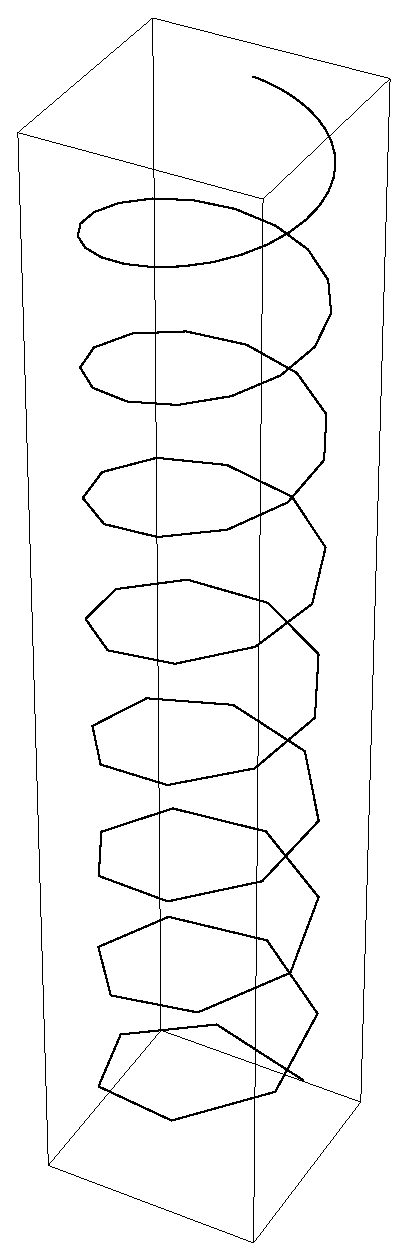
\epsfig{file=position.eps,width=6cm}
\end{center}

\newpage

\section*{Parallel Processing}
Parallel processing is basically running exactly the same program (process) on multiple CPU's.  Each process knows its number and how many CPU's are present and can thus do different work.  Messages are then passed between processes as required by the algorithm.

MPI is one of several message passing implementations.  Good references for MPI

\hspace{1cm}\code{http://nf.apac.edu.au/training/MPI/}

\hspace{1cm}\code{http://nf.apac.edu.au/training/MPI/MPI\_1.1/mpi-report.html}

A very basic MPI program looks like

\fcode{src/firstmpi.f90}

The first command in an MPI program is ALWAYS \code{MPI\_Init}.  It is not defined what should happen before this.  The last command is \code{MPI\_Finalize}.  Again, it isn't defined what should happen after this.  \code{MPI\_COMM\_WORLD} is defined in \code{mpif.h} and defined the communicator or ``world'' that we are transmitting message in.

\newpage

To compile and run the code is very simply.  Notice how each process no does something slightly difference.

\small
\begin{verbatim}
sc1: > f90 firstmpi.f90 -o firstmpi -lmpi
sc1: > prun -n 4 ./firstmpi
Process:  0/ 4
Process:  1/ 4
Process:  2/ 4
Process:  3/ 4
sc1: > 
\end{verbatim}
\normalsize

The above example doesn't require any communication.  The simplest form of communication is the \code{MPI\_Send} and \code{MPI\_Recv} which will allow us to send and receive messages.

\fcode{src/pingpong.f90}

We can look at the \code{man} page for \code{MPI\_Send} to see what the arguments to the subroutines are.  Note: the arguments are in ``c-style'' so you need to make the appropriate change to Fortran.

\small
\begin{verbatim}
MPI_Send(3)                          MPI                          MPI_Send(3)

NAME
  MPI_Send -  Performs a basic send

SYNOPSIS
  #include "mpi.h"
  int MPI_Send( void *buf, int count, MPI_Datatype datatype, int dest,
         int tag, MPI_Comm comm )

INPUT PARAMETERS
  buf  - initial address of send buffer (choice)
  count
       - number of elements in send buffer (nonnegative integer)
  datatype
       - datatype of each send buffer element (handle)
  dest - rank of destination (integer)
  tag  - message tag (integer)
  comm - communicator (handle)

NOTES
  This routine may block until the message is received.

NOTES FOR FORTRAN
  All MPI routines in Fortran (except for MPI_WTIME and MPI_WTICK ) have an
  additional argument ierr at the end of the argument list. ierr is an
  integer and has the same meaning as the return value of the routine in C.
  In Fortran, MPI routines are subroutines, and are invoked with the call
  statement.

  All MPI objects (e.g., MPI_Datatype , MPI_Comm ) are of type INTEGER in
  Fortran.
\end{verbatim}
\normalsize

\newpage

This simple little code will pass pass the process rank to the rank+1 process and receive a message from the rank-1 process.  Notice how I avoid grid lock by getting alternate processes to send/receive and then vice versa.

\small
\begin{verbatim}
sc1: > f90 pingpong.f90 -o pingpong -lmpi
sc1: > prun -n 4 ./pingpong
 3/ 4    sent:  3    recv:  2
 0/ 4    sent:  0    recv:  3
 1/ 4    sent:  1    recv:  0
 2/ 4    sent:  2    recv:  1
sc1: > 
\end{verbatim}
\normalsize

\newpage

\section*{Exercise}
Two charged particles interact via the coulomb force
\begin{equation}
F=\frac{q Q}{4\pi\epsilon_{0} \mathbf{r}^{2}}
\end{equation}

Using a simple $2^{nd}$ order method, write a program to simulate $n$ particles in a box, where $n$ is read in from an input file.  The box should have hard walls which don't remove any energy from the particles.  Ensure the energy (kinetic and potential) of the system is conserved.  Plot the motion of a small number of particles in Matlab or Mathematica.



%\section*{Makefile}

%When developing code, there can be many modules, libraries, include files and other pieces that need to be included in the compilation of the main program.  Compiling the various pieces of the code and main program, after a modification, can often require many steps with complicated dependancies.  One method to keep track of the project is a \makefile.

%Quite simply, this file defines which pieces of code depend on other pieces and how to build each piece.  The \makefile can also perform many other pre-compile requirements like constructing the appropriate directory structure and checking for avaliable libraries.  It also allows your code to be compiled by another user without any knowledge of how the code needs to be built.

%\newpage

%For further information see the man page for \code{make}:

%\begin{verbatim}
%NAME

%  make - Maintains up-to-date versions of target files and performs shell
%  commands

%SYNOPSIS

%  make [-bemNqrtUuxy] [-c  | -C] [-F  | -i  | -k  | -S] [-n  | -p  | -s] [-f
%  makefile] [macro_definition...] target...

%  The make command updates one or more target names by executing commands in
%  a description file.

%STANDARDS

%  Interfaces documented on this reference page conform to industry standards
%  as follows:

%  make:  XCU5.0

%  Refer to the standards(5) reference page for more information about indus-
%  try standards and associated tags.

%OPTIONS

%  -b  Has no effect; exists so that older-version make dependency files con-
%      tinue to work.  This option is on by default.
%\end{verbatim}

%\newpage

%A \makefile also allows the compile options and build procedure to be modified easily.  Perhaps the largest advantage of using \code{make} and a \makefile is the reduction in typing and work.

%\fcode{Makefile}

%\newpage

%\small
%\begin{verbatim}
%sc0: > gmake particle
%if ( test ! -d bin ) then ( mkdir bin ) fi
%if ( test ! -d obj ) then ( mkdir obj ) fi
%f95 -I./obj -DDOUBLE -fpp -module obj -fast -speculate all -c src/precision.f90
% 	-o obj/precision.o
%f95 -I./obj -DDOUBLE -fpp -module obj -fast -speculate all -c src/globals.f90
% 	-o obj/globals.o
%f95 -I./obj -DDOUBLE -fpp -module obj -fast -speculate all -c src/inout.f90
% 	-o obj/inout.o
%f95 -I./obj -DDOUBLE -fpp -module obj -fast -speculate all -c src/newtons.f90
% 	-o obj/newtons.o
%f95 -I./obj -DDOUBLE -fpp -module obj -fast -speculate all -c src/propagation.f90
% 	-o obj/propagation.o
%f95 -I./obj -DDOUBLE -fpp -module obj -fast -speculate all -c src/particlepropagate.f90
% 	-o obj/particlepropagate.o
%f95 -fpp -module obj -fast -speculate all -I./obj -DDOUBLE obj/precision.o 
%	obj/globals.o obj/inout.o obj/newtons.o obj/propagation.o obj/particlepropagate.o
% 	-o bin/particle 
%sc0: > cat input.dat
%time=            1.0d0
%time steps=      100
%b=               0.5d0 -2.0d0 1.0d0
%velocity=        5.0d0 0.7d0 -1.0d0
%position=        0.0d0 0.0d0 0.0d0
%mass=            1.0d0
%charge=          1.0d0
%accuracy=        1.0d-6
%end

%sc0: > bin/particle 
% t=   0.000000000000000E+000     energy=    13.2450000000000     
% t=   1.000000000000000E-002     energy=    13.2450000006223     
% t=   2.000000000000000E-002     energy=    13.2450000105794     
% .
% .
% .
% t=   0.980000000000000          energy=    13.2456394939767     
% t=   0.990000000000000          energy=    13.2456526807577     
% t=    1.00000000000000          energy=    13.2456651651549     
%sc0: > gmake clean
%rm -f obj/*
%rm -f bin/*
%sc0: > 
%\end{verbatim}
%\normalsize

%\newpage

%\begin{center}
%
\epsfig{file=velocity.eps,width=6cm}

%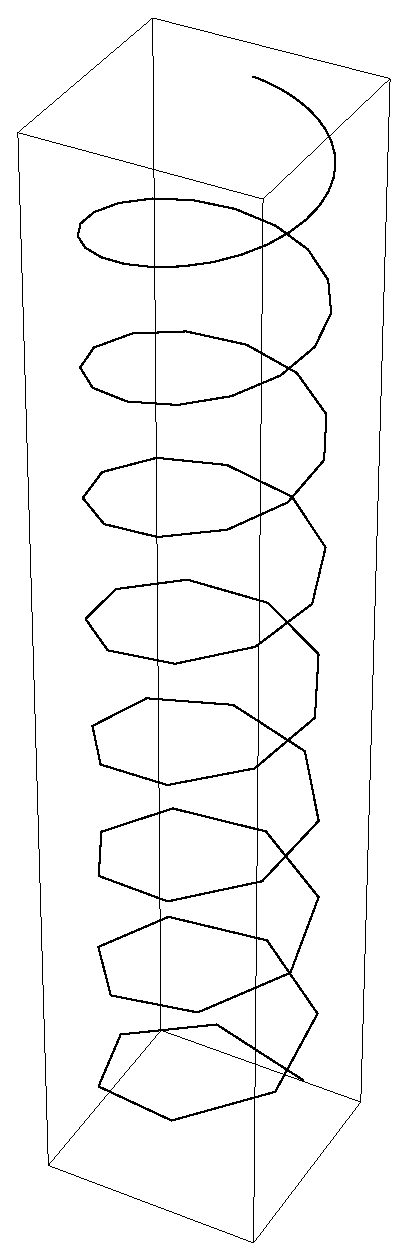
\epsfig{file=position.eps,width=6cm}
%\end{center}

%\newpage

%\section*{Automatic parallelisation}

%As a first step, code can be automatically made to run in parallel on the \SC by using the KAP automatic precompiler.  This precompiles your code putting in compiler directives to tell the compiler how to parallelise your code.  Simply use \code{kf90} rather than \code{f90} when compiling.

%\begin{verbatim}
%################################################################################
%#
%#  Define some useful variables
%#

%FORTRAN =			kf90

%FLAGS =				-fkapargs='-conc -ur=1'

%DEFINES =			-DDOUBLE

%LIBRARIES =			

%INCLUDES =			-I./obj
%\end{verbatim}

%Notice how easy it is to adjust the code for recompilation using a \makefile .  The \code{kf90} compiler produces \code{.cmp.f90} files which contain the compiler directives for use with OpenMP

%\begin{verbatim}
%C$OMP PARALLEL IF (M .GT. 20) SHARED (M,LL1,DY,N,DX,U,ERROR) PRIVATE (J,
%C$OMP& YY,I,XX,TEMP,ERROR1)
%       ERROR1 = 0D0
%C$OMP DO 
%       DO J=1,M
%        IF (LL1) THEN
%         YY = -1D0 + DY * DBLE (J - 1)
%         DO I=1,N
%          XX = -1D0 + DX * DBLE (I - 1)
%          TEMP = U(I,J) - (1. - XX * XX) * (1. - YY * YY)
%          ERROR1 = ERROR1 + TEMP * TEMP
%         END DO
%        END IF
%       END DO
%C$OMP END DO NOWAIT
%C$OMP CRITICAL (II1)
%       ERROR = ERROR + ERROR1
%C$OMP END CRITICAL (II1)
%C$OMP END PARALLEL 
%\end{verbatim}

%\newpage

%The to run the code, tell the computer how many threads to use and execute.

%\begin{verbatim}
%sc0: > setenv OMP_NUM_THREADS 1
%sc0: > timex ./jacobp < input.1
% Total Its :         2001 l2 Error :   2.031111084176103E-008
% Solution Error :   8.496940324632936E-004

%real   17.6
%user   17.5
%sys    0.0
%sc0: >setenv OMP_NUM_THREADS 4
%sc0: >timex ./jacobp < input.1
% Total Its :         2001 l2 Error :   2.031111084176072E-008
% Solution Error :   8.496940324632975E-004

%real   4.9
%user   19.1
%sys    0.4
%sc1: > 
%\end{verbatim}

\end{document}